Samotný program je rozdělen do několika podadresářů a souborů. Adresářová struktura s popisem nejdůležitějších adresářů a souborů je ukázána na obrázku~\ref{fig:adresare}. Klíčový soubory je {\tt data\_preparation.py}, kde je proveden {\it preprocessing} vstupních dat. Dalšími důležitými souborem jsou soubory {\tt runoff.py} a {\tt time\_step.py} zde je samotné řešení modelu. Soubory v adresáři {\tt main\_clasess/} obsahují definici datových struktur jednotlivých řešených dějů a skládají dohromady metody k řešení jednotlivých dějů modelu. Tuto metody jsou pak definované v adresáři {\tt processes/}. 

Program SMODERP je napsaný v jazyce Python. Python je často používaný GIS softwary jako skriptovací jazyk a jsou pro ně k dispozici knihovny pro efektivní práci s geodaty\footnote{knihovna arcpy pro ArcGIS či knihovny grass.script pro GRASS GIS}. Programy či skripty napsané pomocí Python jsou spustitelné v prostředí daných GIS softwarů. Současná verze modelu SMODERP používá Python 2.7.X, který je kompatibilní s ArcGIS 10.X.

Na obrázku~\ref{fig:flowchart} je zjednodušený diagram toku programu. Program řeší v každém časovém kroku rovnici~\ref{eq:bilancnirce}. Pokud je překročena kritická výška a půda se začne vymílat, začne se do celkového  odtoku  započítávat i rýhoví odtok. Bilanční rovnice je rozšířena (rovnice~\ref{eq:bilancnircerill}). Pokud je řešená buňka tok, načítá se celkový přítok $\sum_j^m \acs{oin}_{j,t-1}$ (případně $\sum_k^n \acs{oinrill}_{k,t-1}$) v rovnici~\ref{eq:bilancnirce} (~\ref{eq:bilancnircerill}) do daného úseku toku, kde se odtok řeší pomocí Chezyho rovnice.

Pokud v daném časovém kroku překročí rychlost v jakékoli buňce Courantovo kritérium dojde ke zmenšení časového kroku a výpočet se v daném kroku opakuje. Pokud je Courantovo kritérium nízké, je možné časový krok zvýšit. To odpovídá kontrole a aktualizaci časového kroku v diagramu na obrázku~\ref{fig:flowchart}. Po dosažení konečného času dojde k uložení výsledných hodnot a ukončení programu.




\begin{figure}[t!]
  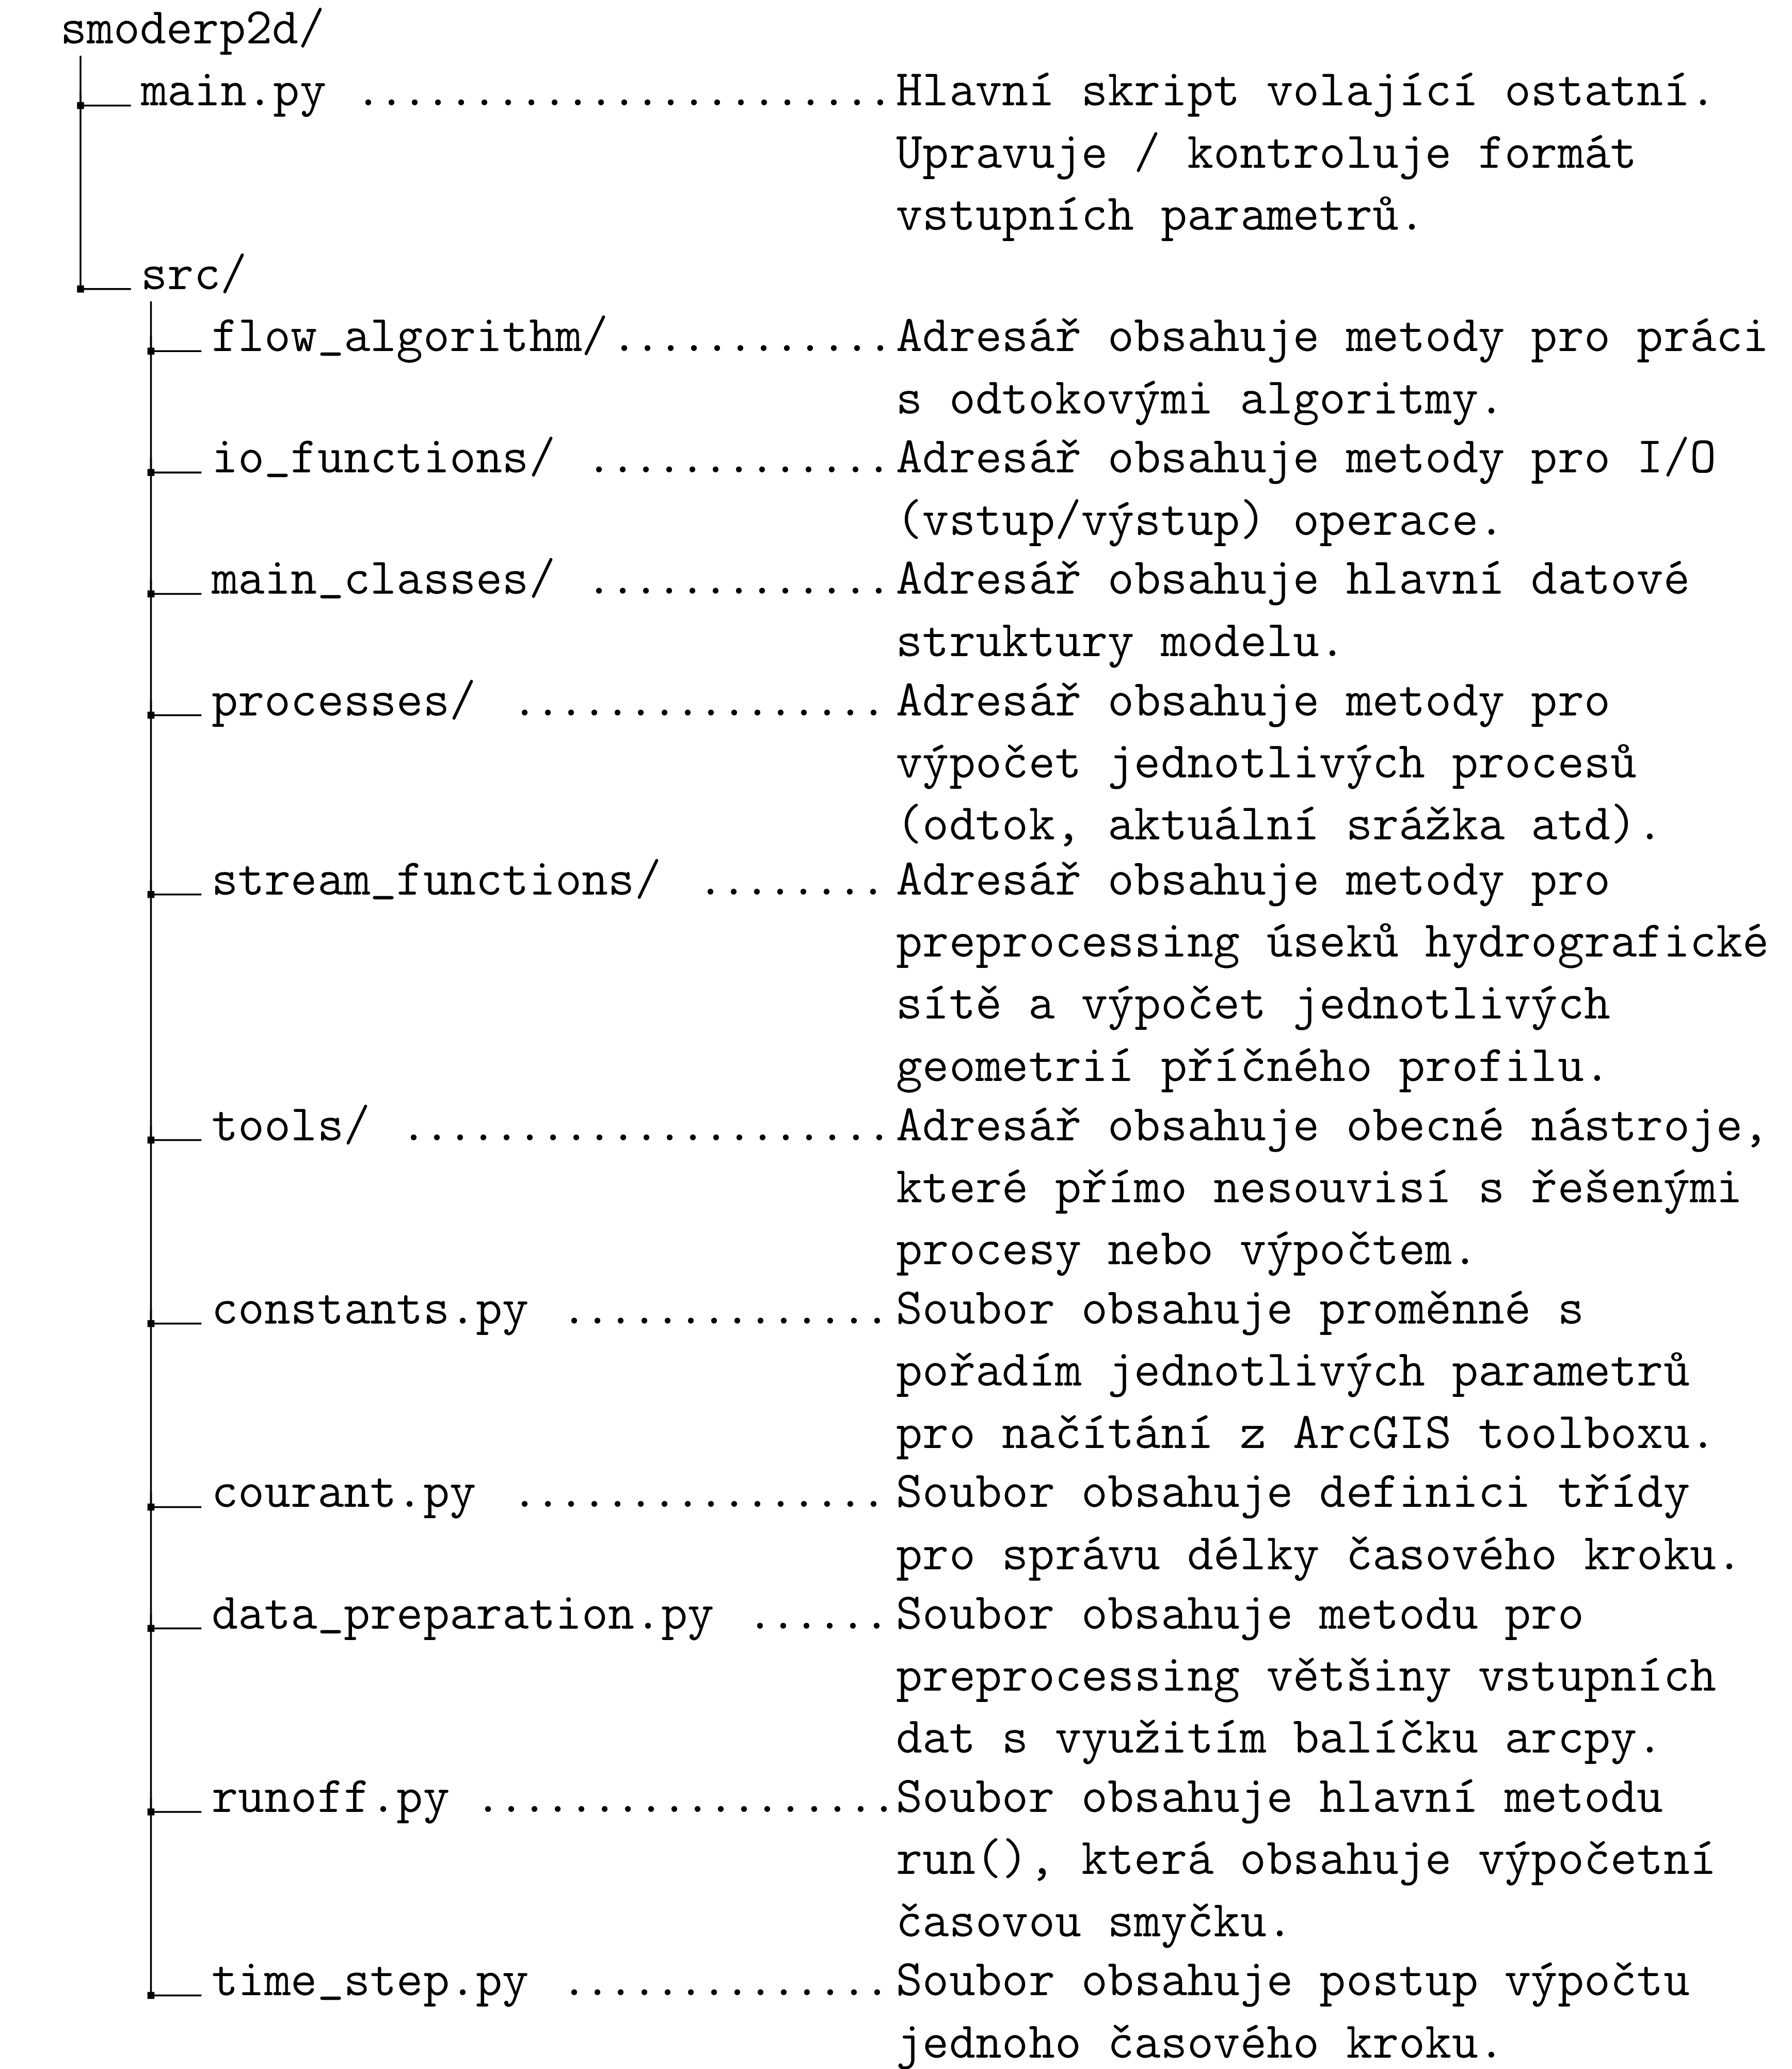
\includegraphics[width=0.8\textwidth]{./img/dirtreenapng.png}
  \caption{důležité soubory a adresáře modelu \smod}
  \label{fig:adresare}
\end{figure}






% 
% \begin{itemize}
% \item main.py
% \item constants.py
% \item rainfall.py
% \item functions.py
% \item runoff.py
% \item data preparation.py
% \end{itemize}
% 

% \textbf{z diplomky:}
% Samotný model je spouštěn je ze souboru main.py, kde podle zvoleného typu výpočtu je importován příslušný soubor. V současnosti se jedná o soubor runoff.py. Na začátku je provedena příprava dat. Jedná se o soubor data preparation.py. Jádrem přípravných prací je vytvořit ze vstupních dat rozsah řešeného území a vytvořit vrstvu směrů přítoků do jednotlivých buněk. V souboru constants.py jsou označeny vstupy. Soubor functions.py shromažďuje funkce, které se v programu opakují, aby je bylo možno znovu snadněji použít. Soubor rainfall.py převede vstupní textový soubor srážkové události na jednotlivé úhrny podle časového kroku modelu. Samotný výpočet probíhá v jádru souboru runoff.py. Pro jednotlivé časové kroky je vypočítáván povrchový odtok. Výpočet probíhá rozdílně na dvou typech buněk. Plošný odtok je počítán v buňkách, kde hladina nepřekročila hladinu kritickou pro soustředění odtoku a rýhový odtok na buňkách, kde tato hranice překročena byla. Výpočet probíhá ve vícerozměrných maticích. Výsledkem jsou rastry, polygonové vrstvy a textové soubory.




% \textbf{doplnit}
% \begin{itemize}
% \item že se vstupy natahují z AG
% \item časový cyklus
% \item plnění matic a jak je to v matici zapsáno
% \item práce s elementama
% \item co si model pamatuje do dalšího kola
% \item testování výpočtu CLF
% \end{itemize}
% 
% \begin{large}
% \textbf{Někde najité texty}
% \end{large}

% Objektově orientované zpracování toku programu umožňuje jednak lepší orientaci v kódu a také lepší běh programu. Jednotlivé procesy jsou ro
\subsection{Programovací jazyk Python} \label{sec:python}
  Python je objektově orientovaný programovací jazyk, který se může využít v~mnoha oblastech vývoje softwaru. Nabízí významnou podporu k~integraci s~ostatními jazyky a~nástroji a~přichází s~mnoha standardními knihovnami. Jeho použití je velice široké od~programů na~zpracování multimedií až~po~zpracování textů. Python není závislý na~platformě, na~které běží \cite{python}. Zajímavým rozšířením jazyka Pyhton je NumPy. Je to balíček užívaný pro~vědecké výpočty. Umožňuje podporu velkých, multi-dimenzionálních polí a~matic, spolu s~velkou knihovnou matematických funkcí pro~práci s~těmito poli \cite{numpy}. Pomocí tohoto balíčku bylo v~programu operováno s~naprostou vetšinou polí a~matic. V~současnosti (Prosinec 2013) je nejnovější verze jazyka 3.3.3. Poslední verze vývojové větve 2.x Pythonu vyšla v~roce 2010 a~byla to~verze 2.7. Nyní všechna vylepšení jazyka už jsou dělána pro~vývojovou větev 3.x. K~tvorbě programu byla zvolena verze 2.6.5, která~je kompatibilní s~programem ArcGIS~10.0.     

  
  
  
  
  
  
\subsection{CFL podmínka - řešení nestability výpočtu} \label{sec:cfl}
  V předchozím verzích programu SMODERP nebyla ošetřena podmínka stability výpočtu, která vychází z explicitního řešení časově derivace. Při větších rychlostech toku či nevhodně zvolené délce časového kroku došlo k situaci, kdy z buňky odteklo více vody než v ní bylo. Situace byla nazvána přetečení. Program se ukončil a uložil se poslední úspěšný časový krok. 

  V současné verzi programu SMODERP 2D je tento problém vyřešen Courant-Friedrich-Lewy (\acs{CFL}) podmínkou. Splnění této podmínky zajišťuje konvergenci explicitního řešení pokus je platí, že $\acs{CFL} < 1.0$. Z obecné rovnice CFL podmínky byla odvozena a upravena podmínka pro účely modelu SMODERP 2D na následující tvar:
  \begin{equation}
    \acs{CFL} = \frac{1}{0.5601}\frac{v \acs{dT}}{\acs{dX}} 
    \label{eq:courrovnice}
  \end{equation}
  \begin{tabular}{rrl}
    kde \jj{CFL}{,}
        & $v$ & je rychlost plošného či rýhového toku, \\
        \jj{dT}{\ a}
        \jj{dX}{.}
  \end{tabular}
  
  Po dopočítání časového kroku je uložena nejvyšší hodnota \acs{CFL} zjištěná z {\bf plošného odtoku} pomocí vztahu~\ref{eq:courrovnice}. Poté se porovná s kritickou hodnotou a podle pravidel znázorněných v tabulce~\ref{tab:cflsheet} se změní (nebo nezmění) délka časového kroku \acs{dT}. Pokud dojde ke změně \acs{dT} opakuje se výpočet v daném časovém. Do dalšího času se výpočet posune, až když je zaručena stabilita výpočtu. 
  
  \begin{table}[t!]
    \centering
    \caption{Kritéria změny časového kroku vycházející z plošného odtoku}
    \label{tab:cflsheet}
    \begin{tabular}{ccc}
      \hline
        nové  &  $\acs{CFL} < 0.75 \lor 1.0 < \acs{CFL}$ & $ 0.75 \geq \acs{CFL} \geq 1.0 \lor \acs{CFL} = 0.0^*$ \\
        \hline
        \hline
        \acs{dT} &  = $MIN(\frac{0.5601\acs{dX}}{v};\acs{dTmax})$ & = původní \acs{dT}\\
        \hline
%         \multicolumn{3}{l}{{\small \acs{CFL} = 0.0 zpravidla v případně, pokud je rychlost proudění nulová. Potom nelze }}
    \end{tabular}
  \end{table}

  Proudění v {\bf rýhách} je zpravidla řádově rychlejší než plošný odtok. Pokud bychom v tomto případě uplatňovali stejný princip jako u plošného odtoku, časový krok by byl musel být velmi malý čímž by se prodlužoval strojoví čas výpočtu. K odtoku v rýhách většinou nedochází na celém území, ale pouze v poměrně malém počtu buněk (v poměru k celé ploše výpočetní oblasti). Proto se při výpočtu rýhového odtoku přistoupilo k lokálnímu krácení časového kroku pouze v buňkách, kde k rýhovému odtoku skutečně dojde. Časový krok v rýhách je dělen celočíselně faktorem označeným jako \acs{ratio}. CFL číslo se proto ukládá zvlášť u plošného a zvlášť u rýhového odtoku. Ke změně časového kroku plošného odtoku dojde pokud $\acs{ratio} > 10$. Časový krok plošného odtoku je pak násoben multiplikátorem \acs{dTmult}, který se po každém překročení maximální  \acs{CFL} zmenší na 90 \% své dosavadní hodnoty. Pokud je \acs{CFL} příznivé multiplikátor \acs{dTmult} se postupně zvětšuje vždy o 10 \% na hodnoty 1. Pravidla pro změna faktoru \acs{ratio} a multiplikátoru \acs{dTmult} jsou shrnuty~\ref{tab:cflrill}.
  \begin{table}[t!]
    \centering
    \caption{Kritéria změny faktoru \acs{ratio} při dělení časového kroku pří výpočtu rýhového odtoku}
    \label{tab:cflrill}
    {\small
    \begin{tabular}{llll}
      \hline
        nové  &  $\acs{CFL}_{rill} < 0.3 $ & $ 0.5 < \acs{CFL}_{rill}$ & $ 0.3 \geq \acs{CFL}_{rill} \geq 0.5 $ \\
        & & & $\lor \acs{CFL}_{rill} = 0.0 $ \\
        \hline
        \hline
        \acs{ratio} &  = $MAX(\acs{ratio} - 1;1)$ &  = $MIN(\acs{ratio} + 1;10)$ & = původní \acs{ratio}\\
                     &                              &  pro \acs{ratio} = 10  &                            \\
        \acs{dTmult} &  = $MIN((1/0.9)\acs{dTmult};1)$ &  = $0.9\acs{dTmult}$ & = původní \acs{dTmult}\\
        \acs{dT}    &  & \multicolumn{2}{l}{= $\acs{dT}\acs{dTmult}$} \\
        \hline
        
    \end{tabular}
    }
  \end{table}
  
  
  Obrázek \ref{fig:cfl1} a \ref{fig:cfl2} ukazují chování časového kroku v případě, že je řízen plošným obrázek~\ref{fig:cfl1} nebo rýhovým odtokem obrázek~\ref{fig:cfl2}. 
  
  
  \begin{figure}%[h!]
    \centering
    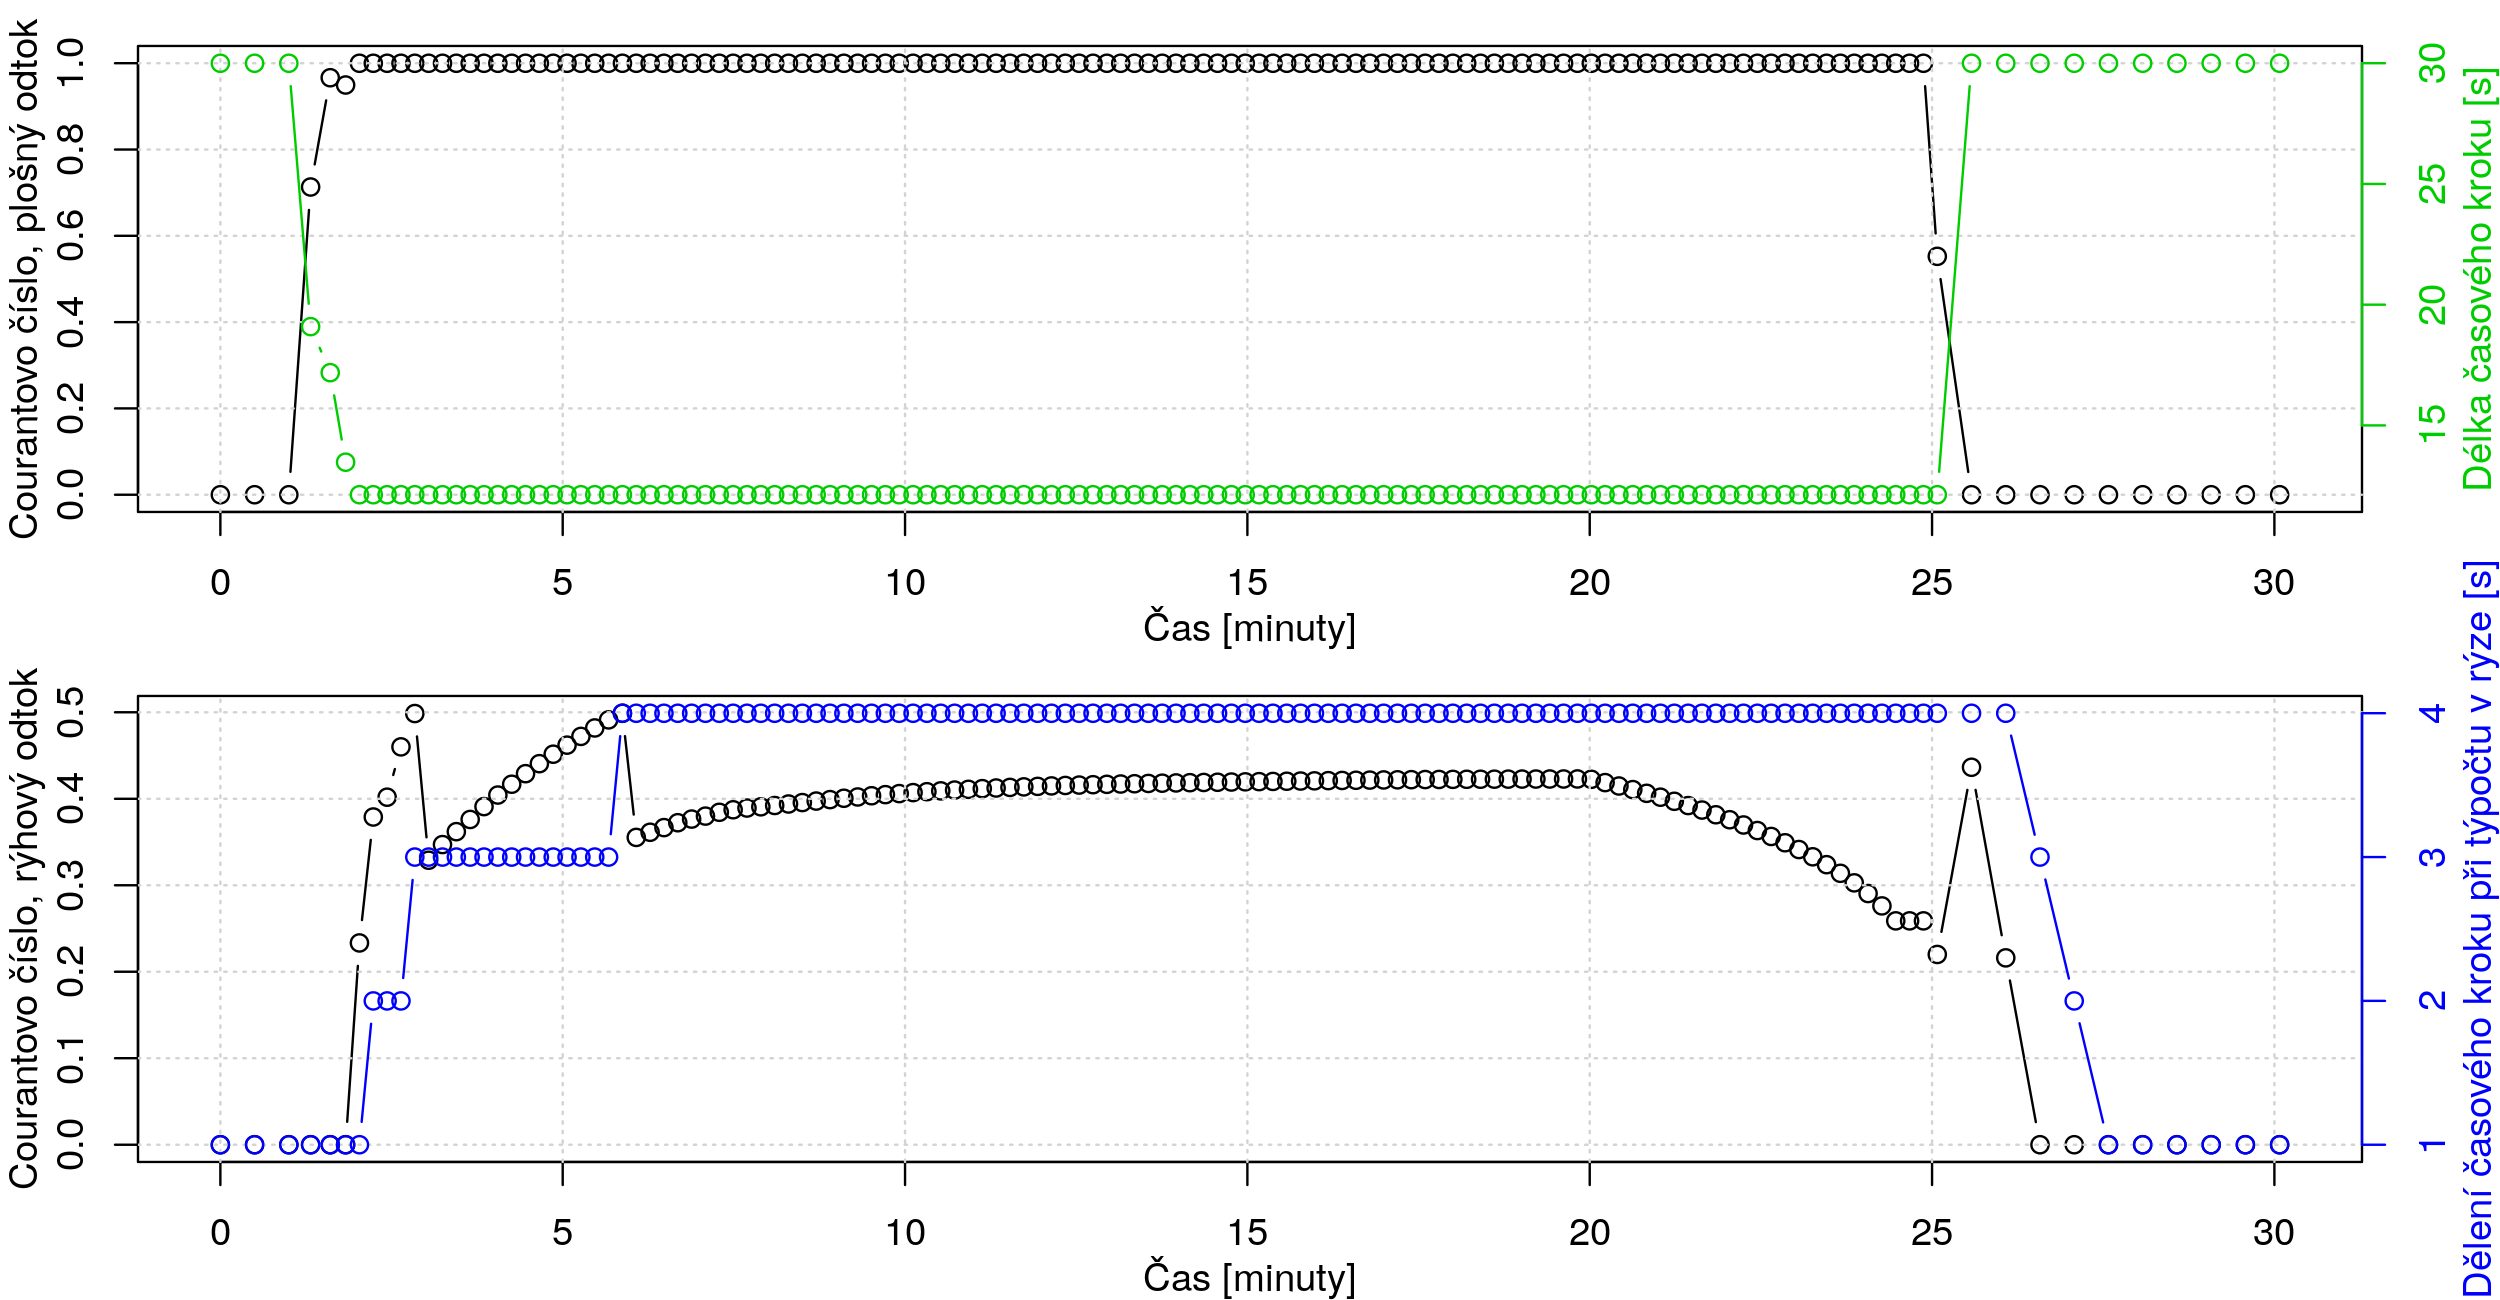
\includegraphics[width=1.0\textwidth]{./img/courantratio.png}
    \caption{Časový krok řízen rychlostí plošného odtoku. \acs{CFL} rychle stoupne k 1 a začne zkracovat časový krok (horní graf). Pár minut později $\acs{CFL}_{rill}$ stoupne nad 0.5, \acs{ratio} stoupne na 2 (dolní graf) tím začne lokálně dělit časový krok při výpočtu rýhového odtoku. \acs{ratio} na spodním grafu stoupne maximální na 4 a neovlivní tedy celkový časový krok (na horním grafu). Na obou grafech je vidět jak se po 25 minutě (kdy v modelu skončila srážková událost) dálka časového kroku i \acs{ratio} vrátí na původní hodnoty.}
    \label{fig:cfl1}
  \end{figure}
  
  
  \begin{figure}%[h!]
    \centering
    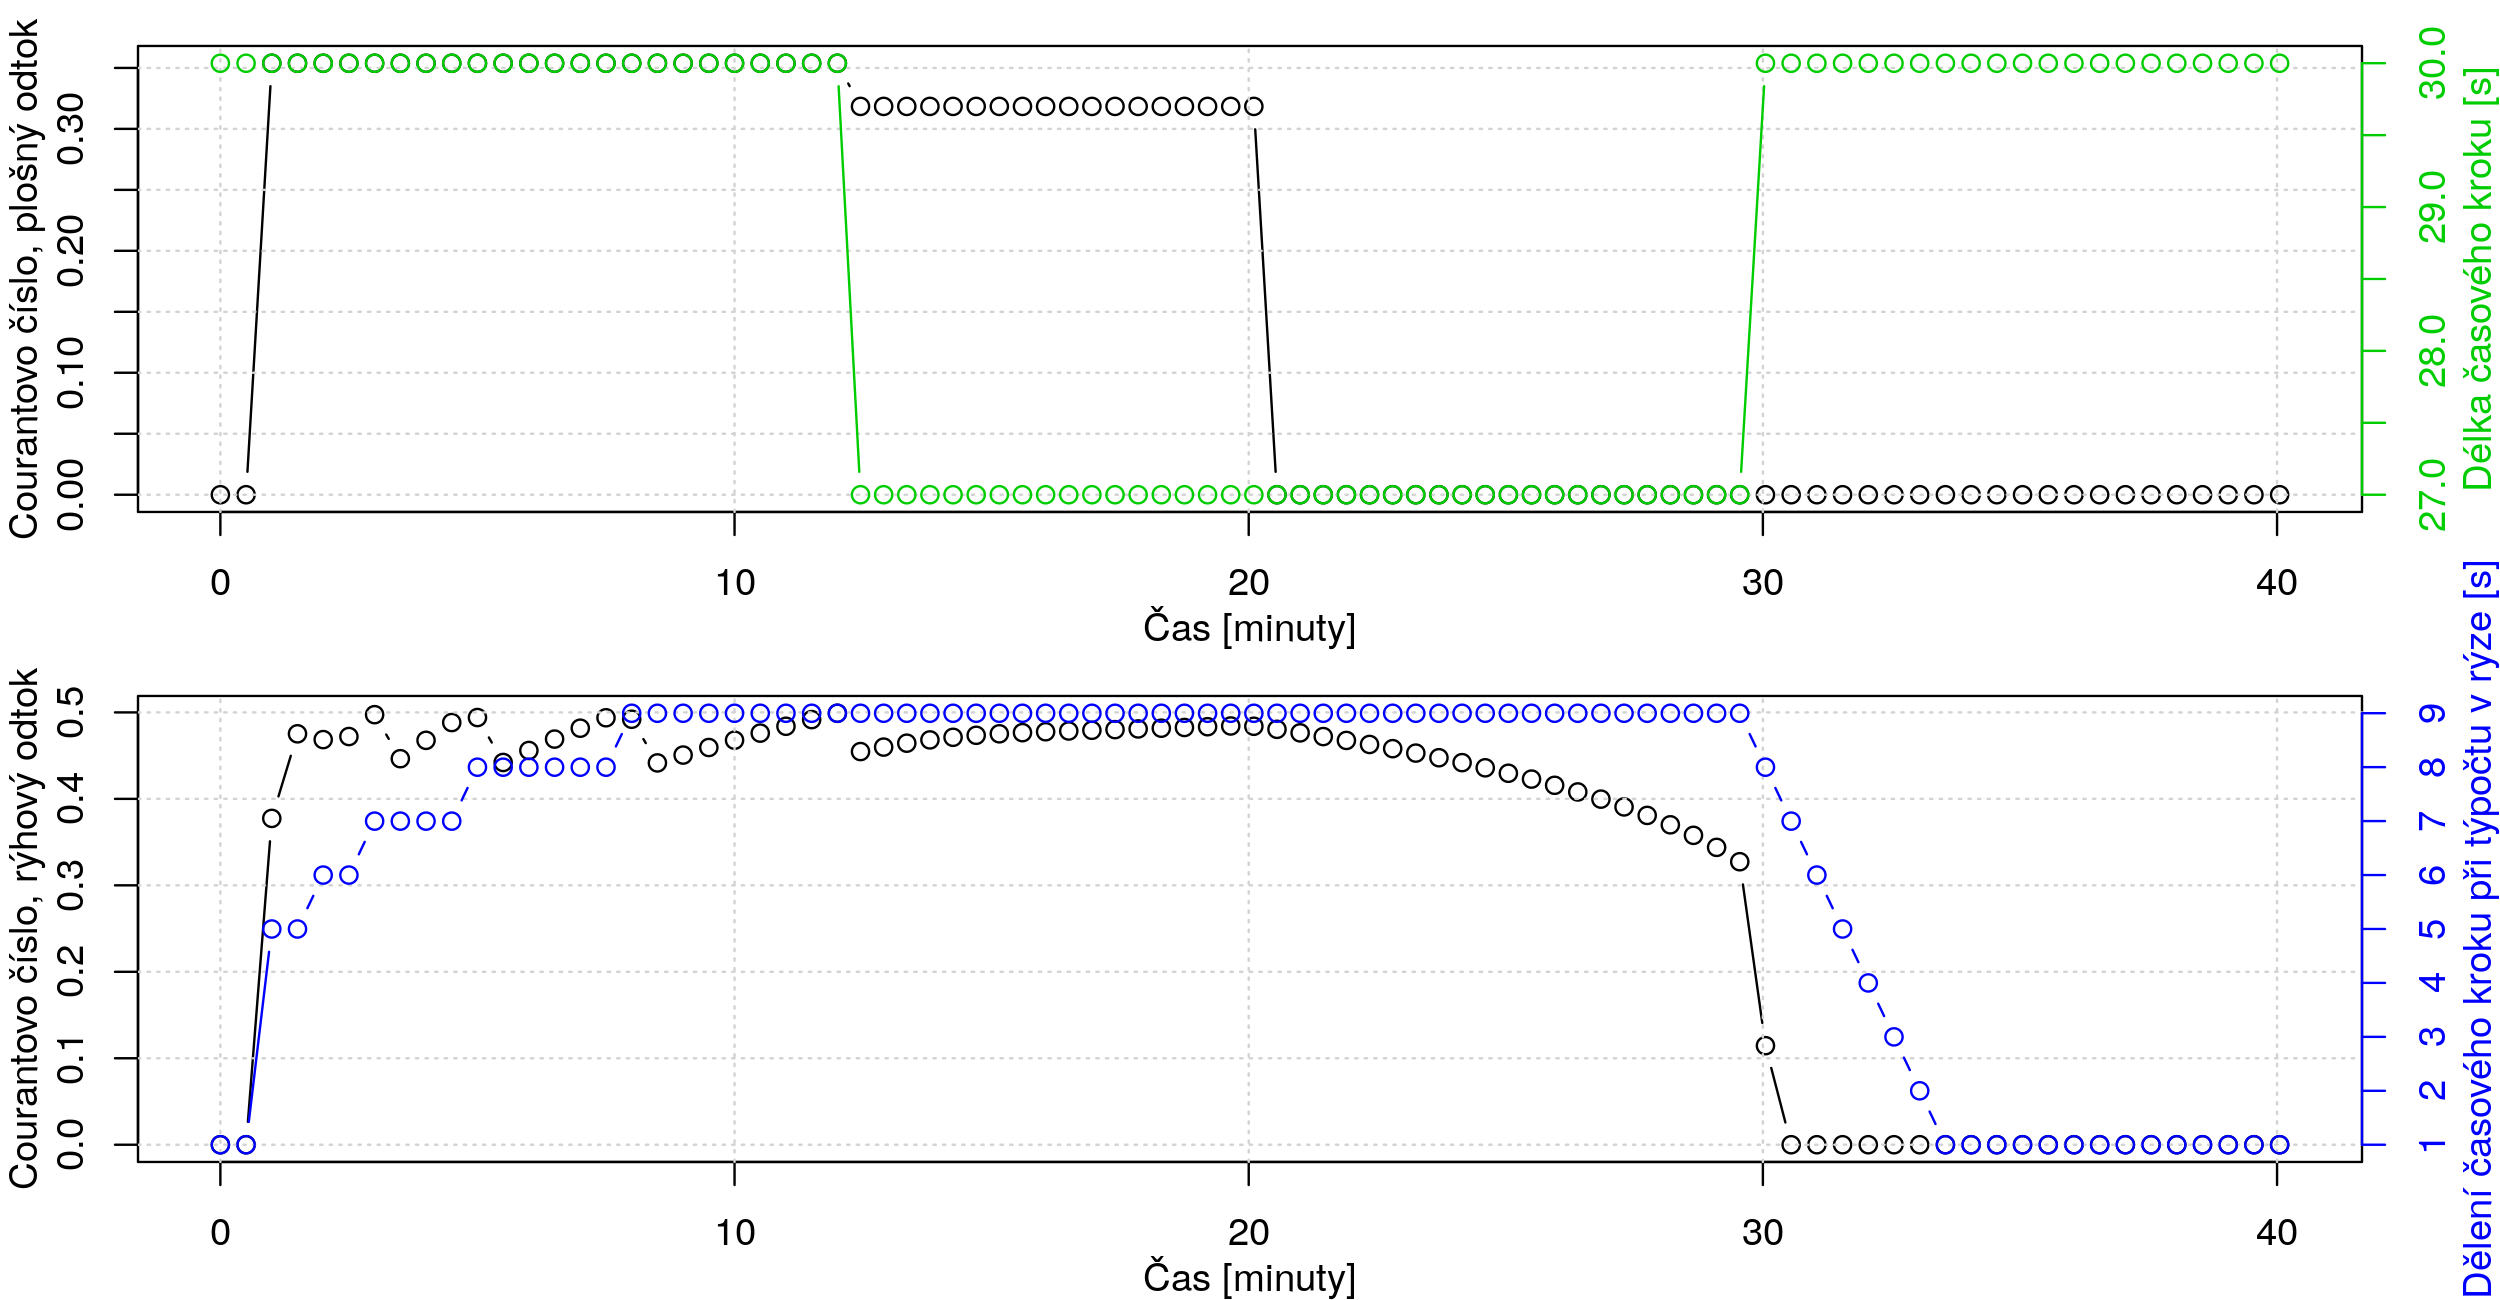
\includegraphics[width=1.0\textwidth]{./img/courantratio2.png}
    \caption{Časový krok řízen rychlostí rýhového odtoku.  \acs{CFL} plošného odtoku nepřekročí během výpočtu hodnotu cca 0.35 (na horním grafu), proto nemá žárný vliv na velikost časového kroku.  $\acs{CFL}_{rill}$ rychle vystoupí 9 krát nad kritickou hodnotu 0.5 (spodní graf, prvních 10 minut výpočtu). To způsobí nárůst \acs{ratio} na 9 což je maximální povolené dělení lokálního časového kroku při výpočtu rýhového odtoku. Pří dalším překročení hodnot 0.3 (cca 12 minuta na dolním grafu) dojde ke zmenšení celkového časového kroku na 90 \% původní hodnoty (horní graf). Na obou grafech je vidět jak se po 20 minutě (kdy v modelu skončila srážková událost) dálka časového kroku i \acs{ratio} vrátí na původní hodnoty.}
    \label{fig:cfl2}
  \end{figure}
  

% Hlavní myšlenkou řešení nestability výpočtu je zmenšení časového kroku při náznaku, že by mohlo dojít k přetečení. Pro každý časový krok je podle rovnice \ref{courrovnice} vypočteno v každé buňce Courantovo číslo $C$. Dále je určeno maximum Courantova čísla ve všech buňkách v časovém kroku. Toto číslo je zásádní, jelikož podle něj se porovnává, zda je situace potencionálně nebezpečná a bude potřeba zmenšit časový krok. Na změnu časového kroku byla použita funkce pojmenovaná $courant$:

% Dochází k porovnání, zda se Courant pohybuje v rozmezí hodnot 0.8 a 1.0. Pokud je hodnota vyšší, je zmenšen časový krok  a pokud je hodnota nižší, časový krok se zvýší. Nikdy však nemůže být výšší než původní časový krok zadaný. Testování probíhalo tak, aby podmínka zmenšila co možná nejméně časový krok a při tom nedošlo k numerické nestabilitě v kroku následujícím. Velikost časového kroku $\Delta t$ zásadně ovlivňuje dobu běhu celého modelu. Čím více se zmenší časový krok, tím déle trvá modelu než doběhne do požadové časové hodnoty a ukončí se. V současné verzi je největším problémem fakt, že při větších průtocích na větším území dojde brzy ke zmenšení $\Delta t$ na velmi nízkou hodnotu, např. 0.01 minuty a tím se úměrně zvyšuje časová náročnost výpočtů.




\begin{figure}[t!]
{\small
\begin{center}
\begin{tikzpicture}[node distance=1.5cm]


\node (start) [startstop] {Start};
\node (dataprep) [process, below of=start] {Příprava dat};
\node (in) [io, left of=dataprep, xshift=-4.0cm] {Vstupní data};

\node (dec1) [decision, below of=dataprep, yshift=-0.5cm] {Konečný čas?};

\node (atm) [process, below of=dec1, yshift=-0.5cm] {Srážka za \acs{dT}};
\node (flow) [process, below of=atm] {Plošný odtok};


\node (check) [process, right of=flow, xshift=2.0cm] {Kontrola \acs{dT}};
\node (updatet) [process, right of=atm, xshift=2.0cm] {Aktualizace \acs{dT}};

\node (dec2) [decision, below of=flow, yshift=-0.5cm] {{\footnotesize Překročení kritické výšky hladiny?}};
\node (rillflow) [process, below of=dec2, yshift=-0.5cm] {Rýhový odtok};

\node (dec3) [decision, below of=rillflow, yshift=-0.5cm] {Je buňka v toku?};
\node (streamflow) [process, below of=dec3, yshift=-0.5cm] {Odtok úsekem toku};

\node (output) [io, below of=streamflow, yshift=-0.5cm] {Výstupní data};
\node (stop) [startstop, below of=output, yshift=-0.5cm] {Konec};

% uzly ohnutym caram
\node (dd1) [guide, right of=rillflow, xshift=2.0cm] {};
\node (dd2) [guide, right of=dec1, xshift=2.0cm] {};
\node (dd3) [guide, right of=dec2, xshift=2.0cm] {};
\node (dd4) [guide, right of=dec3, xshift=2.0cm] {};
\node (dd5) [guide, right of=streamflow, xshift=2.0cm] {};
\node (dd6) [guide, left  of=dec1, xshift=-2.0cm] {};
\node (dd7) [guide, left  of=output, xshift=-2.0cm] {};


% jednotlive sipky
\draw [arrow] (start) -- (dataprep);
\draw [arrow] (in) -- (dataprep);
\draw [arrow] (dataprep) -- (dec1);
\draw [arrow] (dec1) -- node[anchor=west] {ne} (atm);
\draw [arrow] (atm) -- (flow);
\draw [arrow] (flow) -- (dec2);
\draw [arrow] (dec2) -- node[anchor=west] {ano} (rillflow);
% \draw [arrow] (dec1) -- node[anchor=north] {ano} (output);
\draw [arrow] (output) -- (stop);
\draw [arrow] (rillflow) -- (dec3);
\draw [arrow] (dec3) -- node[anchor=west] {ano} (streamflow);
\draw [arrow] (check) -- (updatet);


% ohnute cary line (jen cara) do guide (jen neviditelny bod)
%             arrow  z guide (jen neviditelny bod) tam kam chci

\draw [line] (updatet) -- (dd2);
\draw [arrow] (dd2) -- (dec1);

\draw [line] (dec2) -- node[anchor=north] {ne}(dd3);
\draw [arrow] (dd3) -- (check);

\draw [line] (dec3) -- node[anchor=north] {ne}(dd4);
\draw [arrow] (dd4) -- (check);

\draw [line] (streamflow) -- node[anchor=north] {}(dd5);
\draw [arrow] (dd5) -- (check);


\draw [line] (dec1) -- node[anchor=north] {ano}(dd6);
\draw [line] (dd6) -- (dd7);
\draw [arrow] (dd7) -- (output);



\end{tikzpicture}
\end{center}
}
\caption{Flow chart toku programu}
\label{fig:flowchart}
\end{figure}
